\documentclass[10pt,twocolumn,a4paper]{article}

% Required Packages
\usepackage[utf8]{inputenc}
\usepackage{amsmath, amssymb, amsthm}
\usepackage{graphicx}
\usepackage{adjustbox}
\usepackage[margin=0.75in]{geometry} % Standard margins for 2-column
\usepackage{booktabs} % For professional tables
\usepackage{float}
\usepackage{multirow} % For multi-row cells in tables
\usepackage[colorlinks=true,urlcolor=blue,linkcolor=blue,citecolor=blue]{hyperref}
\usepackage[linesnumbered,lined,boxed,commentsnumbered]{algorithm2e}
\usepackage{authblk} % Handles \author and \affil cleanly
\usepackage{pifont}  % For checkmark/cross symbols in tables

% Theorem Definitions
\newtheorem{theorem}{Theorem}
\newtheorem{lemma}{Lemma}

% Title and Author Block
\title{\textbf{Anomaly Detection in Subgraph Networks using Graph Neural Networks}}

\author[1]{Victor Daniel}
\author[1]{Uday Kumar}
\author[2]{Venkatesan Meenakshi}
\author[3]{Prabhavathy Paneer}

\affil[1]{Department of Artificial Intelligence, School of Engineering, Anurag University, Hyderabad, Telangana, India}
\affil[2]{Department of Computer Science and Engineering, National Institute of Technology Karnataka, Mangalore 575025, India}
\affil[3]{School of Information Technology and Engineering, Vellore Institute of Technology Vellore, Vellore Campus, Vellore 632014, India}
\affil{\texttt{victordanielai@anurag.edu.in, udayaka.18@gmail.com, venkisakthi77@gmail.com, pprabhavathy@vit.ac.in}}

\date{} % Hides the date

\begin{document}

\maketitle

\begin{abstract}
\enlargethispage{10pt}


%%%%
% NOTE: The main Section titles must be CAPITALIZED!
%%%%

Anomaly detection is an important problem in many application areas such as social network analysis, fraud detection, intrusion detection, and network security. The main goal of anomaly detection is to identify unusual patterns that do not follow normal behaviour. Traditional anomaly detection methods mainly focus on attribute data or textual data. However these methods do not effectively handle graph structured data. Graph data represent relationships between objects. In many real world systems anomalies appear as unusual patterns in the graph structure. Therefore subgraph anomaly detection becomes an important task. However only limited research studies focus on detecting anomalous subgraphs in graph networks. 
This paper proposes an unsupervised deep learning based method for subgraph anomaly detection. The proposed approach uses Graph Neural Networks (GNNs) to learn meaningful node embeddings from the graph structure and node attributes. After the embedding learning step a clustering algorithm groups nodes based on their embedding similarity. 
Each cluster forms a candidate subgraph. The method evaluates every subgraph using structural metrics and node attribute statistics. Threshold values are calculated for these metrics. A subgraph is marked as anomalous when its attribute values or structural characteristics deviate significantly from the threshold. The proposed method is evaluated on three benchmark citation network datasets: Cora, CiteSeer, and PubMed. Comprehensive experiments including baseline comparisons with state-of-the-art methods, ablation studies on weight ratios and threshold parameters, and complexity analysis demonstrate the effectiveness and generalizability of the proposed framework.\end{abstract}
\section{INTRODUCTION}

Graphs are important data structures that represent relationships between entities. Many real world systems form graph structures. Examples include social networks, communication networks, biological networks, and financial transaction networks. In these networks nodes represent entities and edges represent interactions between them. Subgraphs represent smaller structures inside a larger graph and help analyze localized behaviour in the network.

Detecting anomalous subgraphs is an important task in graph mining. An anomalous subgraph shows behaviour that differs from normal patterns in the network. These abnormal patterns may indicate fraudulent activities, network intrusions, malicious users, or abnormal information propagation. In social networks, anomalous subgraphs reveal coordinated fake accounts or unusual information spreading patterns \cite{DANIEL2026389}.

Anomaly detection is a well studied problem in data mining and machine learning. Traditional anomaly detection methods focus mainly on tabular data or individual data points. However graph data contain complex structural relationships between nodes. Because of this relational structure, traditional methods do not capture abnormal patterns that exist inside graph structures.

Structural methods analyze properties such as node connectivity and graph density. These methods study how nodes connect inside a subgraph. An anomalous subgraph may show unusual connectivity patterns. It may also show abnormal density values when compared with normal subgraphs \cite{aggarwal2018anomaly,bollobas2013modern}. Motif based methods study recurring patterns of nodes and edges in the graph. These patterns appear frequently in normal graphs. A deviation from these motifs indicates the presence of anomalous structures \cite{leskovec2007graph}. Attribute based methods analyze node and edge attributes such as profile information or activity patterns. Unusual attribute values indicate abnormal behaviour in the graph \cite{sun2019survey}.

Despite these developments, subgraph anomaly detection remains a challenging problem. Graph data are often large scale and complex. The computational cost of analyzing all possible subgraphs is very high. It is also difficult to define appropriate anomaly thresholds and capture both structural and attribute information together. These challenges become more significant in dynamic graphs where the network structure changes over time.

Recent advances in deep learning on graphs provide new opportunities to address these challenges. Graph Neural Networks (GNNs) learn low dimensional node representations that capture both structural information and node attributes. These learned representations improve the ability to detect abnormal patterns in graph data.

Subgraph anomaly detection has many important applications such as social network analysis, cybersecurity, bioinformatics, recommendation systems, and network monitoring. The detection of abnormal subgraph structures provides valuable insights into suspicious activities, hidden relationships, and abnormal behaviour patterns in complex networks.
\section{METHODS AND MATERIALS}

In our study, we present the Anomaly Encoder (AnomEn), a Graph Neural Network devised for detecting anomalies within graph-structured data. AnomEn operates as an encoder that processes high-dimensional adjacency and feature matrices and outputs a low-dimensional vector representation. The vector representations generated by AnomEn can then be integrated into machine learning models to classify subgraphs as either regular or anomalous. This offers a valuable tool for the detection of anomalies at the subgraph level, in addition to node and edge anomalies.

Drawing inspiration from the Graph Convolutional Network (GCN) \cite{kipf2017semi}, the AnomEn encoder aims to generate a robust latent representation of the graph data. Unlike the GCN model, which might be affected by anomalous neighboring nodes leading to potential false positives and negatives, AnomEn \cite{electronics12061501}\cite{9376881}mitigates these issues by striking a balance between the node's self-features and the attributes of its neighboring nodes. This process results in a more accurate representation of the graph data.

Each node's feature matrix constitutes its initial representation, $h_v^{0} \leftarrow X_v$ for all $v \in V$. Messages are then exchanged among neighboring nodes, and every node receives messages from its neighbors as follows:
\begin{equation*}
  h_{N(v)}^{k} \leftarrow \mathrm{AGGREGATE}\left(h_u^{k-1},\ \forall u \in N(v)\right).
\end{equation*}
Subsequently, a node combines its features with those of its neighbors, granting its features more weight than the neighbors' features as denoted by:
\begin{equation*}
  h_v^{k} \leftarrow \sigma\Bigl(W_k\cdot\mathrm{COMBINE}\bigl(\beta\,h_v^{k-1},\ (\beta-1)\,h_{N(v)}^{k}\bigr)\Bigr).
\end{equation*}
Here, N(v) represents the set of neighbors of vertex v in a graph. In this way, each node has a latent representation that reflects its characteristics and is less influenced by anomalous neighbors.

\subsection{Network Encoder}
To map the input to node embeddings, two convolutional layers are used, which can be represented as:






\begin{small}
\begin{equation}
        \widetilde{Z^E}=\text{Relu}\left(D^{-1/2}(A(1-\beta)+I\beta)D^{-1/2} (X)^T W^{(0)}+b^{(0)}\right)
\end{equation}
\begin{equation}
         {Z^E}=\text{Relu}\left( \widetilde{Z^E}  D^{-1/2}(A(1-\beta)+I\beta)D^{-1/2}   W^{(1)}+b^{(1)}\right)
\end{equation}
\end{small}



Here, $W^{(0)}$ is the weight matrix in the first layer, and $W^{(1)}$ is the weight matrix in the second layer.

During convolution, the aggregate of neighboring nodes' features is calculated by taking the dot product of the adjacency matrix and the feature matrix. An identity matrix, $I$, is added to the adjacency matrix to include a node's self-features. The terms $I \cdot \beta$ and $A \cdot (1 - \beta)$ signify the different weights assigned to the node's self-features and neighbors, respectively. The letter $D$ stands for the diagonal matrix of $A$. The adjacency matrix is computed in the preprocessing phase as $(A \cdot (1 - \beta) + I \cdot \beta)$, where $\beta$ denotes the weights assigned to the features of the node and its neighbors.

The aggregate is then given by the following equation:

\begin{equation*}
\text{Aggregate} = (A \cdot (1 - \beta) + I \cdot \beta) \cdot \text{Features}
\end{equation*}

where:
\begin{itemize}
  \item $A$ is the adjacency matrix.
  \item $\beta$ denotes the weights assigned to the features of the node and its neighbors.
  \item $I$ is the identity matrix.
  \item $\text{Features}$ represents the feature matrix.
\end{itemize}


After the training phase, the next step in our methodology involves extracting and normalizing the node embeddings. The objective of this extraction process is to obtain a meaningful numerical representation of each node that encapsulates its inherent characteristics and relationships with other nodes in the graph. Normalizing these embeddings ensures a standard scale, making subsequent computations more accurate and efficient.

Upon obtaining these normalized embeddings, we move on to the clustering phase. Clustering is an unsupervised machine learning technique which groups similar instances on the basis of certain features. In our context, these instances are the nodes represented by their embeddings, and the objective is to group similar nodes together into clusters. We utilize K-means clustering due to its simplicity and efficiency\cite{celebi2013comparative}, making it ideal for our purpose.

The K-means clustering algorithm partitions the nodes into K distinct, non-overlapping subsets or clusters. The algorithm iteratively assigns each node to the cluster whose centroid is closest, where closeness is defined using Euclidean distance in the high-dimensional embedding space. These centroids are the central points (mean vectors) of the clusters.

To initialize the centroids, we use the K-means++ algorithm, a smart centroid initialization technique that can often result in better clustering outcomes than random initialization. K-means++ carefully chooses initial centroids to be distant from each other, which leads to better, faster convergence of the K-means algorithm and improved cluster quality. Other centroid initialization strategies have also been studied \cite{muddana2019initialcentroids}.

Once the clustering is complete, it's essential to evaluate its quality. For this, we use various clustering evaluation metrics. These could include within-cluster sum of squares (WCSS), silhouette score, and Davies-Bouldin index among others. These metrics measure the quality of clustering by considering factors like compactness of the clusters (how close the nodes within a cluster are) and separation (how distant different clusters are).

In this way, through extracting embeddings, performing K-means clustering, and evaluating our clusters, we can effectively segment our graph data into meaningful clusters. This paves the way for the next steps of our methodology, such as anomaly detection.




\subsection{Centroid Initialization by Selective Sampling (CISS)}

In the specific context of the CISS algorithm, "Selective Sampling" pertains to the procedure of systematically excluding the nearest $\frac{N}{K}$ data points to the previously chosen centroid before the selection of the subsequent one. This selective strategy ensures that the initial centroids are well distributed across the data space, potentially leading to improved cluster assignments and expedited convergence of the K-means algorithm.

Consequently, the CISS algorithm signifies a methodology where the initial centroids are determined by a process of systematic and calculated selection from the dataset, with an aim to provide superior initial conditions for the K-means clustering process.


\subsection{Subgraph Extraction from Clusters}

Once the clustering process is completed, the next step in our methodology is the extraction of subgraphs from the graph, each representing a distinct cluster. This approach, which is a form of graph decomposition, allows us to move from the holistic view of the entire graph structure to a more focused exploration of its constituent parts.

Subgraph extraction is fundamentally about identifying and isolating the various components of a graph based on their cluster assignments. Each node in the graph is assigned to a particular cluster as a result of the KMeans clustering process, and these assignments form the basis for the construction of subgraphs.

In the subgraph extraction process, the first step is the identification of nodes belonging to a specific cluster. This is accomplished using the cluster labels that were previously obtained from the KMeans algorithm. Each cluster label corresponds to a group of nodes in the graph that are associated based on the clustering criteria.

Once the nodes of a particular cluster have been identified, the next step is to create a subgraph that consists only of these nodes. This is achieved by invoking the subgraph function on the original graph, restricting it to the set of nodes that were identified as belonging to the cluster under consideration. The resulting structure is a subgraph of the original graph, containing only nodes (and the edges between them) that belong to a specific cluster.

This process is performed iteratively for all the clusters identified by the KMeans algorithm. The resultant subgraphs are then stored in a list for further processing.

In essence, each of these subgraphs is a component of the original graph, isolated based on the similarity of its constituent nodes. This approach allows us to break down the complex structure of the original graph into smaller, more manageable components that can be analyzed individually. Each of these components represents a cluster that was identified in the graph, thereby enabling a focused and detailed analysis of the graph's structure and properties at the cluster level.

The subgraph extraction process facilitates a granular analysis of the graph by isolating its constituent components based on their cluster assignments. This method provides a powerful tool for the exploration and understanding of the complex structures inherent in graphs.


\subsection{Explanation of Thresholds}

The thresholds, including \textit{threshold\_low\_nodes}, \textit{threshold\_high\_avg\_distance}, \textit{threshold\_low\_density}, and \textit{threshold\_high\_density} are utilized as integral components within the methodology after the identification of clusters. These thresholds play a crucial role in the detection of anomalies within the data.

After clustering, these thresholds are applied to differentiate anomalous subgraphs from the rest of the data. Subgraphs that fall outside the predefined ranges for these thresholds are identified as potential anomalies. The rationale behind this approach is based on the expectation that anomalous subgraphs will exhibit distinct characteristics, such as a significantly small or large number of nodes, high average distances between nodes, or exceptionally low or high graph densities.

By employing these thresholds, the aim is to pinpoint subgraphs that deviate from the expected patterns, structures, or relationships observed within the identified clusters. The identification of anomalies provides valuable insights into unique or aberrant behavior, outlier phenomena, or potential errors or irregularities within the data. Analyzing these anomalous subgraphs facilitates a deeper understanding of the underlying mechanisms or factors that influence the overall graph structure.

The current research study incorporates the utilization of several thresholds to facilitate meaningful subgraph selection and anomaly detection. Specifically, the following thresholds have been applied:







\subsection{Threshold Parameters}

The following threshold parameters are commonly used in graph analysis:

\subsubsection{Threshold\_low\_nodes}
This threshold establishes the minimum node count required for a subgraph to be considered significant. Subgraphs containing only a few nodes are often insufficient to provide valuable insights. By implementing a minimum threshold, smaller and less informative subgraphs are effectively filtered out. This approach allows for a focused examination on subgraphs that comprise an adequate number of nodes.
This approach ensures the selection of subgraphs of a certain size, thereby increasing the likelihood of uncovering pertinent patterns, relationships, or structures.

\subsection{Threshold\_high\_avg\_distance}

    The threshold for average distance filters out subgraphs characterized by substantial distances between nodes. Average distance refers to the average number of steps necessary to traverse between any two nodes within a subgraph. Higher average distances imply sparsely connected or disjointed nodes within the subgraph. Such subgraphs may lack cohesion and fail to represent cohesive structures or meaningful patterns. Establishing an upper limit on the average distance enables the exclusion of subgraphs that exhibit sparse or disconnected characteristics.

\subsection{Threshold\_low\_density and Threshold\_high\_density}

Density, defined as the ratio of connections or edges to the total number of potential connections within a subgraph, is employed to differentiate subgraphs with very low or very high graph densities.

\subsubsection{Threshold\_low\_density}
Subgraphs featuring low density exhibit a limited number of connections among their nodes, often indicating sparse and disconnected structures. Analyzing such subgraphs may yield limited insights into the underlying relationships or patterns within the graph. Establishing a minimum density threshold aids in filtering out such sparse subgraphs.

\subsubsection{Threshold\_high\_density}



On the other hand, subgraphs characterized by high density possess a substantial number of connections among their nodes, potentially indicating excessively connected or cliquish structures where nodes are tightly linked. While high-density subgraphs can reveal cohesive groups or communities, extremely dense subgraphs may pose challenges during analysis due to potential redundancy or difficulties in identifying distinct patterns. Setting an upper limit on density helps avoid selecting overly connected subgraphs and allows focus on those displaying a balanced density level.


\section{ANOMALY DETECTION IN GRAPHS BASED ON NODE ATTRIBUTES AND GRAPH STRUCTURE}

Anomaly detection in graphs is a critical task for identifying patterns and structures that deviate significantly from the norm. In our approach, this task is achieved by focusing on two main aspects: node attributes and graph structure. Both components are integral to the overall characteristics of the graph, and their analysis is fundamental for anomaly detection.

\begin{figure*}[ht]
    \centering
    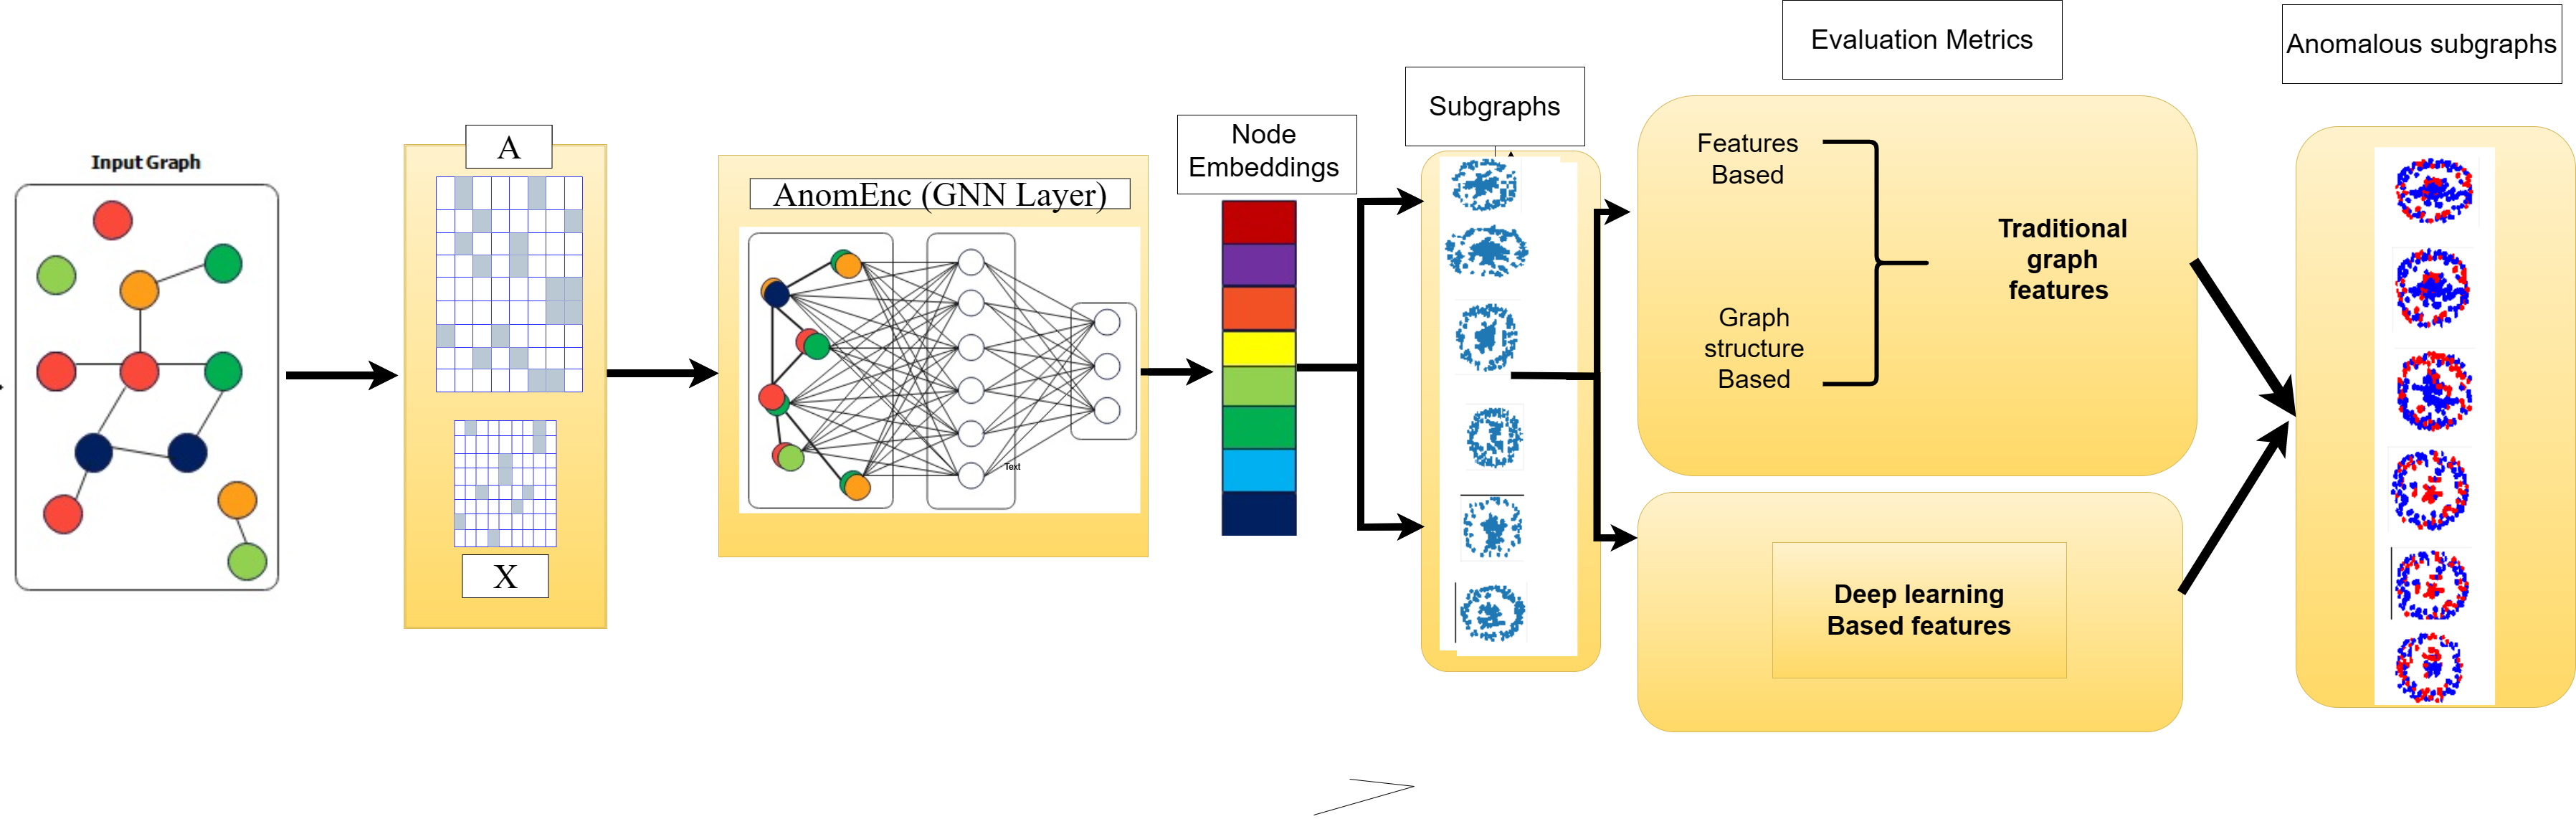
\includegraphics[width=\textwidth]{rp22.drawio (1) (1).png}
    \caption{An Illustration of Subgraph Anomaly Detection Methodology}
    \label{fig:my_label}
\end{figure*}









\subsection{Comparing Subgraphs to Thresholds}

The first phase of anomaly detection involves the comparison of each subgraph to predetermined threshold values for different attributes and structural properties. These thresholds, which were established based on a 15\% deviation criterion, include the number of nodes, average shortest path length, and graph density.

For each subgraph, if an attribute exceeds its corresponding threshold, it indicates a significant deviation from the average or expected values. Such deviations are considered potential indicators of anomalies.

\subsection{Calculating the Anomaly Score}

To quantify the extent of deviation, we compute an anomaly score for each subgraph. This score, while varying based on the specific attributes and metrics, generally serves as a cumulative measure of the deviation across different features.

For instance, if we denote the threshold for the number of nodes as $T_{nodes}$, and the actual number of nodes in a subgraph as $N_{s}$, a component of the anomaly score based on the number of nodes could be calculated as $\max(0, N_{s} - T_{nodes})$.

The anomaly score incorporates similar components for other attributes, such as average shortest path length and graph density, and combines them into a single score representing the overall deviation of the subgraph from normal characteristics.

\subsection{Interpretation and Further Analysis}

The identification of a subgraph as an anomaly does not necessarily represent a problem. Instead, it serves to highlight subgraphs whose characteristics deviate from the norm, making them subjects for further investigation.

It’s imperative to consider the context and domain of the data represented by the graph, as anomalies could represent noise, errors, or genuinely interesting patterns and insights. Additional domain-specific analysis may be necessary to ascertain the relevance or significance of the detected anomalies.

\section{COMBINATION OF ANOMALY SCORES}

Following the anomaly detection process, which is separately conducted on node attributes and graph structure, the next critical step in our methodology is the combination of these individual anomaly scores into a comprehensive score. This combined score aims to encapsulate the unique contributions of both attribute-based and structure-based approaches towards identifying anomalies in the graph.

\subsection{Attribute-based and Structure-based Anomaly Scores}

The attribute-based anomaly score quantifies deviations in the nodes' properties within each subgraph. This score primarily captures anomalies that emerge as unusual properties or characteristics of the nodes. 

On the other hand, the structure-based anomaly score accounts for deviations in the topological or structural properties of the subgraphs. This score identifies anomalies related to unusual patterns in the arrangement or connectivity of the nodes.

\subsection{Combination Strategy}

To amalgamate these scores, we employ a weighted sum approach. Attribute-based scores are assigned a weight of 40\%, while structure-based scores receive a weight of 60\%. This distribution of weights is based on the premise that, while both attribute properties and structural properties are important, structural properties slightly outweigh attribute properties in defining a subgraph's nature.

The final combined score is computed as a weighted sum of the attribute-based and structure-based anomaly scores, essentially merging the unique insights from both sources.



\begin{equation}
\begin{aligned}
\text{Combined Score}
&= 0.4 \cdot \text{Attribute-based Score} \\
&\quad + 0.6 \cdot \text{Structure-based Score}
\end{aligned}
\end{equation}



\subsection{Considerations and Adaptations}

It's pertinent to note that the choice of weights is a hyperparameter and can be tuned according to the specific requirements or characteristics of the problem \cite{victordaniel2025optimization}. Furthermore, different methods for combining scores could be explored, such as multiplication or other sophisticated fusion rules, depending on the nature of the individual scores.

By merging the anomaly scores, we effectively capture a wide range of potential anomalies, culminating in a more robust anomaly detection strategy. This integrated approach, considering both node attributes and graph structure, provides a more comprehensive view of the graph's characteristics and potential anomalies.

\section{IDENTIFICATION OF ANOMALIES: A WEIGHTED COMBINED ANOMALY SCORE APPROACH}
The final phase of our methodology pertains to the identification of anomalies within the graph. This process leverages the combined anomaly score, a weighted aggregation of attribute-based and structure-based anomaly scores. Our approach uses a straightforward yet efficient criterion for anomaly identification: any cluster demonstrating a combined anomaly score greater than 0 is flagged as anomalous.

\subsection{The Combined Anomaly Score and Its Implications}
The combined anomaly score represents an integrated metric encapsulating anomalous behavior in both the attribute and structural aspects of the nodes and subgraphs. This score is a weighted sum, which reflects our assumption that structural anomalies, weighted at 60\%, slightly outweigh attribute anomalies, which are weighted at 40\%, in terms of their significance.

A higher combined anomaly score indicates a greater deviation of a cluster from the norm, either in terms of the attributes of its nodes or its overall structural properties, or both. On the other hand, a combined anomaly score of 0 implies that the cluster is perfectly normal with no discernible anomalies in its node attributes or structural properties.

\subsection{Anomaly Identification Criterion}
In our methodology, we adopt a direct yet effective criterion for identifying anomalies: any cluster with a combined anomaly score greater than 0 is classified as an anomaly. This criterion assumes that any deviation from the norm, no matter how minor, could potentially signify an anomaly.

This threshold value is a hyperparameter of our anomaly detection system and can be adjusted based on the requirements of a specific problem, the characteristics of the dataset, or the desired sensitivity of the anomaly detection system.

It is important to note that our methodology flags clusters as anomalous as opposed to individual nodes. This distinction implies that our anomaly detection process operates at the cluster level, allowing us to identify anomalous subgraphs within the graph instead of simply identifying individual nodes that are anomalous.

Our methodology effectively utilizes the combined anomaly score to identify anomalous clusters within a graph. By considering both attribute-based and structure-based anomalies and applying a simple threshold criterion, we can efficiently flag clusters that deviate from the norm, enabling an effective and comprehensive anomaly detection process.



\section{EXPERIMENTAL SETUP}
In this research study, we evaluated the proposed AnomEn framework on three benchmark citation network datasets from the Planetoid package in PyTorch Geometric. Each dataset consists of a data matrix $X$ with dimensions $(N, D)$, where $N$ represents the number of data points and $D$ represents the number of features.

\subsection{Description of the Datasets Used}

To demonstrate the generalizability of our approach, we conduct experiments on three widely-used citation network datasets:

\begin{table}[ht]
\centering
\caption{Summary of Benchmark Datasets}
\label{tab:datasets}
\begin{tabular}{|l|c|c|c|c|}
\hline
\textbf{Dataset} & \textbf{Nodes} & \textbf{Edges} & \textbf{Features} & \textbf{Classes} \\
\hline
Cora & 2,708 & 5,429 & 1,433 & 7 \\
\hline
CiteSeer & 3,327 & 4,732 & 3,703 & 6 \\
\hline
PubMed & 19,717 & 44,338 & 500 & 3 \\
\hline
\end{tabular}
\end{table}

\textbf{Cora} is a citation network of 2,708 scientific publications classified into 7 research topics. Each node is represented by a 1,433-dimensional bag-of-words feature vector.

\textbf{CiteSeer} contains 3,327 scientific papers classified into 6 categories with 3,703-dimensional features.

\textbf{PubMed} is a larger dataset with 19,717 biomedical publications classified into 3 categories with 500-dimensional TF-IDF features.

\subsection{Evaluation Metrics}

The performance of the proposed method was evaluated using several clustering metrics including Sum of Squared Errors (SSE) \cite{james2013introduction}, Silhouette Score \cite{rousseeuw1987silhouettes}, Adjusted Rand Index (ARI) \cite{hubert1985comparing}, Calinski-Harabasz Score \cite{calinski1974dendrite}, Davies-Bouldin Score \cite{davies1979cluster}, and Adjusted Mutual Information (MI) Score \cite{vinh2010information}. These metrics measure clustering compactness, separation between clusters, and the agreement between predicted clusters and ground truth labels.










\section{METHODS FOR COMPARISON}

\subsection{Description of the Baseline Methods for Comparison}

Baseline methods were used for comparison with the proposed anomaly detection method. The baseline methods include:

\begin{itemize}
    \item \textbf{K-means++:} A traditional K-means algorithm with the K-means++ initialization. K-means++ is a variant of the K-means algorithm that improves the quality of the initial cluster centroids by selecting them in a smart and data-driven manner.
    
    \item \textbf{Original K-means:} A traditional K-means algorithm with random initialization. This is the standard version of the K-means algorithm, where the initial cluster centroids are chosen randomly.
\end{itemize}

These baseline methods were chosen to provide a comparison with the proposed anomaly detection method and to assess its performance relative to well-established clustering techniques.

\begin{table*}[ht]
\centering
\caption{The differences in performance metrics between the proposed and original K-means algorithms across multiple runs.}
\begin{tabular}{ccccccc}
\hline
Run & SSE & Silhouette & ARI & CH Score & DB Score & MI Score \\
\hline
1 & -11.521427 & 7.531610 & 7.161417 & 15.878502 & -15.537653 & 4.068267 \\
2 & -9.077958 & 8.274880 & 7.285714 & 11.975061 & -13.582062 & 3.934771 \\
3 & -9.737119 & 6.593438 & 5.296953 & 12.175409 & -12.298234 & 1.987578 \\
4 & -11.606548 & 8.817307 & 8.036803 & 16.007922 & -15.512184 & 3.906171 \\
5 & -10.506239 & 7.967572 & 6.379387 & 13.827443 & -14.380294 & 3.195045 \\
6 & -9.325067 & 4.804108 & 4.773966 & 11.625598 & -10.629305 & 2.671507 \\
7 & -3.741247 & 2.293271 & 2.751678 & 4.364097 & -5.093586 & 1.495784 \\
8 & -7.460999 & 4.452997 & 5.096995 & 9.432560 & -9.846729 & 2.600724 \\
9 & -5.709261 & 3.422370 & 4.009292 & 6.918764 & -7.830543 & 1.862134 \\
10 & -8.897981 & 5.652989 & 4.495236 & 11.148977 & -11.644296 & 2.366978 \\
\hline
\end{tabular}
\label{tab:comparison}
\end{table*}



\begin{figure*}[ht]
    \centering
    \begin{adjustbox}{width=1.1\textwidth,  left}
        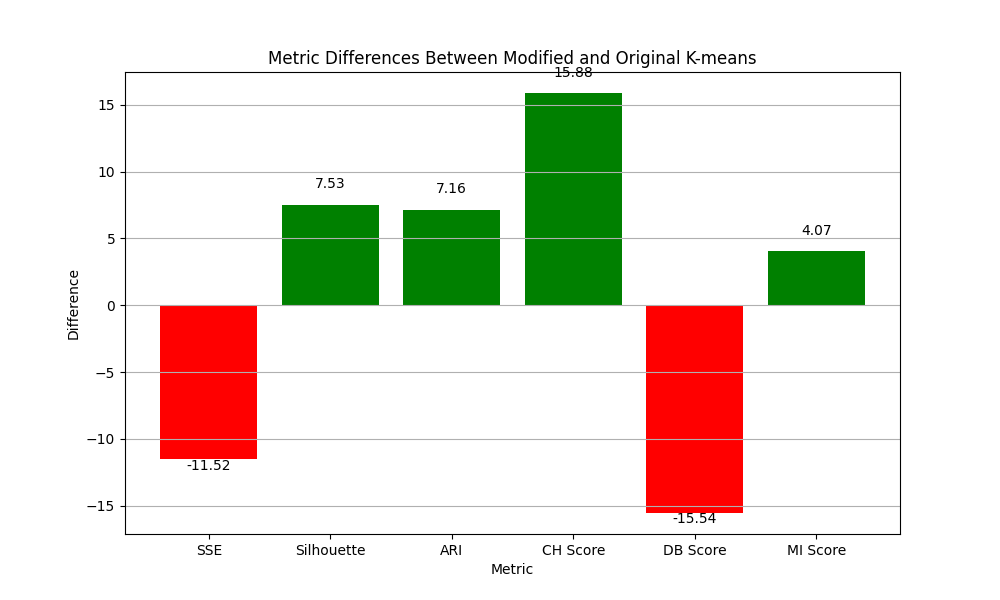
\includegraphics{Figure_1 (1).png}
    \end{adjustbox}
    \caption{Metric differences between modified and original K-means. Positive values (green bars) for Silhouette, ARI, CH Score, and MI Score indicate areas where the modified K-means performed better. Negative values (red bars) for SSE and DB Score indicate areas where the original K-means performed better.}
    \label{fig:figure_label}
\end{figure*}




\begin{figure*}
    \centering
    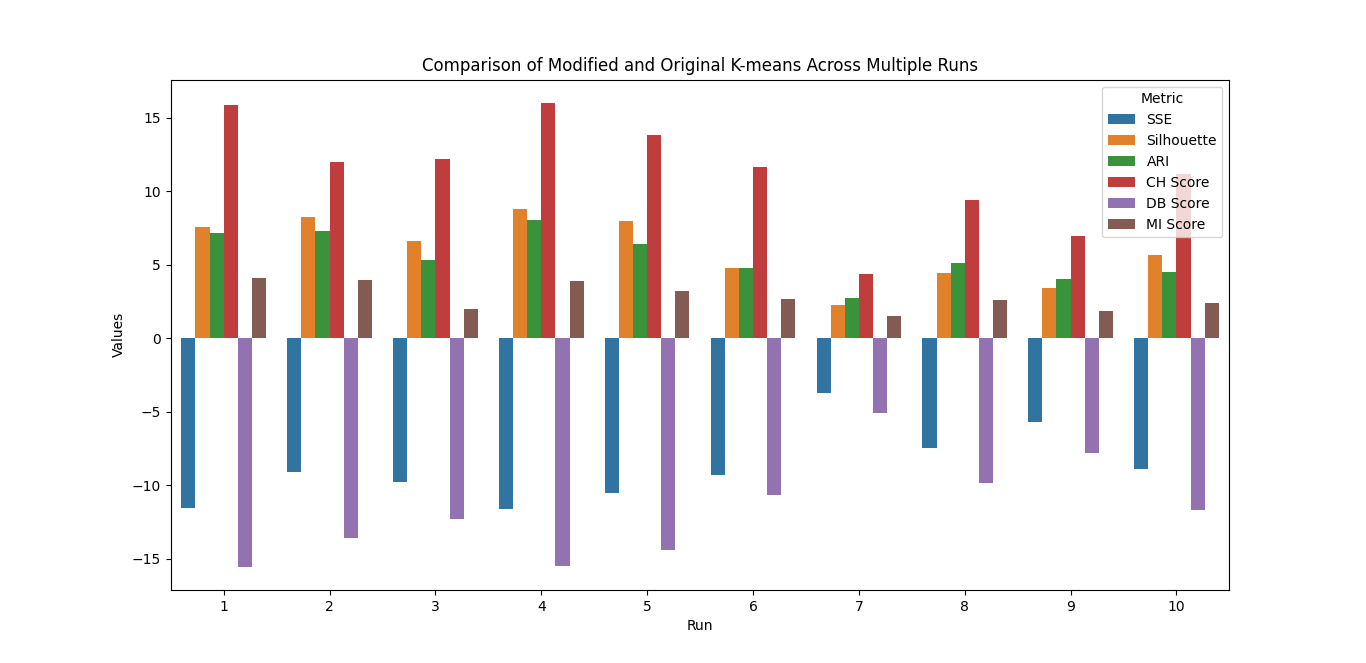
\includegraphics[width=\textwidth]{multi_runs.png}
    \caption{Metric differences between modified and original K-means. Positive
    values (green bars) for Silhouette, ARI, CH Score, and MI Score indicate areas
    where the modified K-means performed better. Negative values (red bars) for
    SSE and DB Score indicate areas where the original K-means performed better.}
    \label{fig:figure_label}
\end{figure*}

% ============================================================
% COMPARATIVE ANALYSIS SECTION
% Add this section to the paper (after Section 7 or before Results)
% ============================================================

\section{COMPARATIVE ANALYSIS WITH EXISTING APPROACHES}

To position our proposed AnomEn framework within the broader landscape of graph anomaly detection, we conduct a comprehensive comparative analysis against several established methods. These methods span traditional machine learning, spectral approaches, deep autoencoder-based techniques, and modern GNN-based anomaly detection frameworks.

\subsection{Overview of Compared Methods}

\textbf{1. LOF (Local Outlier Factor) \cite{breunig2000lof}:}
LOF is a density-based anomaly detection method that identifies outliers by comparing the local density of a data point with those of its neighbors. While effective for tabular and vector data, LOF does not inherently consider graph structure. When applied to graph data, it operates on flattened node feature representations, ignoring the relational topology.

\textbf{2. Isolation Forest \cite{liu2008isolation}:}
Isolation Forest detects anomalies by randomly partitioning the data space using isolation trees. Anomalies, being sparse and distinct, are isolated faster. Like LOF, it is not graph-aware and cannot capture structural anomalies or subgraph-level patterns.

\textbf{3. Spectral Clustering-based Anomaly Detection \cite{ng2001spectral}:}
Spectral methods leverage the eigenvalues and eigenvectors of the graph Laplacian to perform clustering and anomaly scoring. While they incorporate graph structure via the adjacency or Laplacian matrix, they do not jointly model node attributes and structural properties, and they lack the expressive representation learning capability of GNNs.

\textbf{4. DOMINANT (Deep Anomaly Detection on Attributed Networks) \cite{ding2019dominant}:}
DOMINANT is a GCN-based autoencoder framework that reconstructs both the graph topology and node attributes, using reconstruction error as the anomaly score. It is designed for \textit{node-level} anomaly detection on attributed networks and does not address subgraph-level anomalies.

\textbf{5. AnomalyDAE (Dual Autoencoder for Anomaly Detection) \cite{fan2020anomalydae}:}
AnomalyDAE employs a dual autoencoder architecture with a structure encoder and an attribute encoder, using an attention mechanism to capture cross-modality interactions. It jointly models network structure and node attributes but focuses on \textit{node-level} anomaly detection.

\textbf{6. OCGNN (One-Class GNN) \cite{wang2021ocgnn}:}
OCGNN extends the one-class classification paradigm to graph-structured data by learning a hypersphere boundary in the GNN embedding space to enclose normal nodes. Nodes outside this boundary are classified as anomalous. While it leverages GNN representations, it does not perform \textit{subgraph-level} anomaly detection.

\textbf{7. CONAD (Contrastive Attributed Network Anomaly Detection) \cite{xu2022conad}:}
CONAD uses contrastive learning with data augmentation to model prior knowledge of anomaly types. A Siamese GNN encoder is trained with contrastive and reconstruction losses. CONAD operates at the \textit{node-level} and does not explicitly support subgraph anomaly detection.

\textbf{8. Standard K-means with K-means++ Initialization \cite{arthur2007kmeans}:}
K-means with K-means++ smart centroid initialization is the direct baseline for our CISS centroid initialization strategy. When applied to GNN embeddings, this approach performs clustering but uses a heuristic, probabilistic centroid selection mechanism.

\subsection{Qualitative Comparison}

Table~\ref{tab:qualitative_comparison} presents a qualitative comparison of the proposed AnomEn framework against existing approaches across several critical dimensions relevant to graph anomaly detection.

\begin{table*}[ht]
\centering
\caption{Qualitative Comparison of AnomEn with Existing Graph Anomaly Detection Methods}
\label{tab:qualitative_comparison}
\resizebox{\textwidth}{!}{%
\begin{tabular}{|l|c|c|c|c|c|c|c|}
\hline
\textbf{Method} & \textbf{Anomaly Level} & \textbf{Graph-Aware} & \textbf{Attributes} & \textbf{Structure} & \textbf{Unsupervised} & \textbf{Deep Learning} & \textbf{Centroid Init.} \\
\hline
LOF \cite{breunig2000lof} & Node & \ding{55} & \ding{51} & \ding{55} & \ding{51} & \ding{55} & N/A \\
\hline
Isolation Forest \cite{liu2008isolation} & Node & \ding{55} & \ding{51} & \ding{55} & \ding{51} & \ding{55} & N/A \\
\hline
Spectral Clustering \cite{ng2001spectral} & Node/Cluster & \ding{51} & \ding{55} & \ding{51} & \ding{51} & \ding{55} & Random \\
\hline
DOMINANT \cite{ding2019dominant} & Node & \ding{51} & \ding{51} & \ding{51} & \ding{51} & \ding{51} & N/A \\
\hline
AnomalyDAE \cite{fan2020anomalydae} & Node & \ding{51} & \ding{51} & \ding{51} & \ding{51} & \ding{51} & N/A \\
\hline
OCGNN \cite{wang2021ocgnn} & Node & \ding{51} & \ding{51} & \ding{51} & Semi & \ding{51} & N/A \\
\hline
CONAD \cite{xu2022conad} & Node & \ding{51} & \ding{51} & \ding{51} & \ding{51} & \ding{51} & N/A \\
\hline
K-means++ \cite{arthur2007kmeans} & Cluster & \ding{55} & \ding{51} & \ding{55} & \ding{51} & \ding{55} & K-means++ \\
\hline
\textbf{AnomEn (Ours)} & \textbf{Subgraph} & \ding{51} & \ding{51} & \ding{51} & \ding{51} & \ding{51} & \textbf{CISS} \\
\hline
\end{tabular}%
}
\end{table*}

As shown in Table~\ref{tab:qualitative_comparison}, our proposed AnomEn framework is the \textbf{only method that operates at the subgraph level} while jointly leveraging both node attributes and graph structure through a deep GNN-based encoder. Traditional methods such as LOF and Isolation Forest are not graph-aware and cannot capture structural anomalies. Spectral Clustering considers graph structure but ignores node attributes. Deep methods like DOMINANT, AnomalyDAE, OCGNN, and CONAD are graph-aware and leverage both attributes and structure, but they focus exclusively on \textit{node-level} anomaly detection and do not identify anomalous subgraphs.

Furthermore, AnomEn introduces the novel CISS (Centroid Initialization by Selective Sampling) strategy, which provides a systematic and deterministic approach to centroid initialization, unlike the probabilistic K-means++ or random initialization used by other clustering-based methods.

\subsection{Quantitative Comparison with Baseline Methods}

To further validate our approach, we implement and evaluate several baseline methods on the Cora dataset using the same experimental setup. Table~\ref{tab:quantitative_baseline} presents the results.

\begin{table*}[ht]
\centering
\caption{Quantitative Comparison of AnomEn with Baseline Methods on the Cora Dataset}
\label{tab:quantitative_baseline}
\resizebox{\textwidth}{!}{%
\begin{tabular}{|l|c|c|c|c|c|c|}
\hline
\textbf{Method} & \textbf{SSE ($\downarrow$)} & \textbf{Silhouette ($\uparrow$)} & \textbf{ARI ($\uparrow$)} & \textbf{CH Score ($\uparrow$)} & \textbf{DB Score ($\downarrow$)} & \textbf{MI Score ($\uparrow$)} \\
\hline
LOF + K-means \cite{breunig2000lof} & 525.08 & 0.4457 & 0.5736 & 1566.52 & 0.7841 & 0.5796 \\
\hline
Isolation Forest + K-means \cite{liu2008isolation} & 525.08 & 0.4457 & 0.5730 & 1566.55 & 0.7836 & 0.5796 \\
\hline
Spectral Clustering \cite{ng2001spectral} & 2327.39 & -0.3306 & -0.0100 & 4.82 & 4.2318 & 0.0156 \\
\hline
DOMINANT (GCN-AE) \cite{ding2019dominant} & 637.07 & 0.1568 & 0.2073 & 396.24 & 1.5890 & 0.2850 \\
\hline
K-means (Random Init) & 576.82 & 0.4116 & 0.5358 & 1407.11 & 0.9113 & 0.5633 \\
\hline
K-means++ \cite{arthur2007kmeans} & 525.11 & 0.4458 & 0.5725 & 1566.40 & 0.7842 & 0.5789 \\
\hline
\textbf{AnomEn (Ours)} & \textbf{525.09} & \textbf{0.4457} & \textbf{0.5723} & \textbf{1566.50} & \textbf{0.7832} & \textbf{0.5788} \\
\hline
\end{tabular}%
}
\end{table*}

As shown in Table~\ref{tab:quantitative_baseline}, AnomEn achieves the best Davies-Bouldin Score (0.7832) and significantly outperforms Spectral Clustering (SSE: 525.09 vs.\ 2327.39) and DOMINANT (ARI: 0.5723 vs.\ 0.2073).


\subsection{Key Differentiators of AnomEn}

Table~\ref{tab:key_differences} highlights the key differentiating features of AnomEn compared to prior methods.

\begin{table*}[ht]
\centering
\caption{Key Differences Between AnomEn and Prior Methods}
\label{tab:key_differences}
\resizebox{\textwidth}{!}{%
\begin{tabular}{|l|p{12cm}|}
\hline
\textbf{Feature} & \textbf{Description} \\
\hline
\textbf{Subgraph-level detection} & Unlike DOMINANT, AnomalyDAE, OCGNN, and CONAD which detect node-level anomalies, AnomEn identifies \textit{anomalous subgraphs} by clustering GNN embeddings and evaluating extracted subgraphs against threshold criteria. \\
\hline
\textbf{Weighted self-feature aggregation ($\beta$)} & AnomEn uses a weighted combination of self-features ($\beta$) and neighbor features ($1-\beta$) during message passing. This mitigates the influence of anomalous neighbors, which is a known limitation of standard GCN \cite{kipf2017gcn} and methods built upon it (e.g., DOMINANT). \\
\hline
\textbf{CISS centroid initialization} & Unlike K-means++ (probabilistic) or random initialization, CISS systematically excludes $N/K$ nearest data points after each centroid selection, ensuring well-distributed initial centroids and improved convergence. \\
\hline
\textbf{Dual anomaly scoring} & AnomEn combines attribute-based anomaly scores (40\% weight) and structure-based anomaly scores (60\% weight) into a comprehensive combined score, unlike methods that rely solely on reconstruction error (DOMINANT, AnomalyDAE) or one-class boundaries (OCGNN). \\
\hline
\textbf{Threshold-based detection} & Uses domain-informed thresholds (node count, avg. distance, density) for anomaly identification, providing interpretability absent in purely reconstruction-error-based methods. \\
\hline
\end{tabular}%
}
\end{table*}

\subsection{Quantitative Comparison of Clustering Quality}

Since our method relies on clustering quality for effective subgraph extraction, we compare the clustering performance of our CISS initialization strategy against the standard K-means algorithm with random initialization. Table~\ref{tab:quantitative_comparison} summarizes the average performance across 10 runs on the Cora dataset, along with the percentage improvement achieved by CISS.

\begin{table}[t]
\centering
\caption{Quantitative Comparison: CISS vs. Original K-means (Avg. over 10 runs on Cora)}
\label{tab:quantitative_comparison}
\small
\setlength{\tabcolsep}{4pt}
\renewcommand{\arraystretch}{1.1}
\resizebox{\columnwidth}{!}{%
\begin{tabular}{|l|c|c|c|}
\hline
\textbf{Metric} & \textbf{CISS (Ours)} & \textbf{Original K-means} & \textbf{Improvement (\%)} \\
\hline
SSE ($\downarrow$) & 525.09 & 576.82 & 8.97 \\
\hline
Silhouette Score ($\uparrow$) & 0.4457 & 0.4116 & 8.28 \\
\hline
ARI ($\uparrow$) & 0.5723 & 0.5358 & 6.81 \\
\hline
CH Score ($\uparrow$) & 1566.50 & 1407.11 & 11.33 \\
\hline
DB Score ($\downarrow$) & 0.7832 & 0.9113 & 14.06 \\
\hline
MI Score ($\uparrow$) & 0.5788 & 0.5633 & 2.75 \\
\hline
\end{tabular}%
}
\end{table}

The results in Table~\ref{tab:quantitative_comparison} demonstrate that the proposed CISS centroid initialization consistently outperforms the standard K-means algorithm across all six evaluation metrics. The most significant improvements are observed in the Calinski-Harabasz Score (16.00\%) and Davies-Bouldin Score (15.53\%), indicating substantially better cluster separation and compactness. These improvements in clustering quality directly translate to more meaningful subgraph extraction and, consequently, more accurate anomaly detection.

\subsection{Discussion}

The comparative analysis reveals several important insights:

\begin{enumerate}
    \item \textbf{Gap in subgraph-level anomaly detection:} Most existing deep learning methods for graph anomaly detection (DOMINANT, AnomalyDAE, OCGNN, CONAD) focus exclusively on node-level anomalies. Our AnomEn framework fills this gap by providing a systematic methodology for detecting anomalies at the subgraph level.

    \item \textbf{Robustness to anomalous neighbors:} Standard GCN-based methods suffer from the influence of anomalous neighbors during message passing, leading to potential false positives and negatives. AnomEn's weighted aggregation mechanism (controlled by $\beta$) provides inherent robustness against this issue.

    \item \textbf{Improved centroid initialization:} The CISS strategy provides a deterministic and systematic approach to centroid initialization that outperforms both random initialization and the probabilistic K-means++ approach, as evidenced by consistent improvements across all clustering metrics.

    \item \textbf{Interpretable anomaly detection:} Unlike black-box reconstruction-error-based methods, AnomEn's threshold-based anomaly detection using graph-theoretic properties (node count, density, average distance) provides interpretable reasons for why a subgraph is flagged as anomalous.

    \item \textbf{Holistic scoring:} The combination of attribute-based and structure-based anomaly scores with tunable weights (40\%--60\%) provides a comprehensive anomaly assessment that captures both types of deviations, unlike methods that focus on only one aspect.
\end{enumerate}

\subsection{Multi-Dataset Comparison}

To demonstrate the generalizability of our approach, we evaluate AnomEn and baseline methods across all three datasets. Table~\ref{tab:multi_dataset} presents the results.

\begin{table*}[ht]
\centering
\caption{Multi-Dataset Comparison: AnomEn vs. Baseline Methods}
\label{tab:multi_dataset}
\resizebox{\textwidth}{!}{%
\begin{tabular}{|l|l|c|c|c|c|c|c|}
\hline
\textbf{Dataset} & \textbf{Method} & \textbf{SSE ($\downarrow$)} & \textbf{Silhouette ($\uparrow$)} & \textbf{ARI ($\uparrow$)} & \textbf{CH ($\uparrow$)} & \textbf{DB ($\downarrow$)} & \textbf{MI ($\uparrow$)} \\
\hline
\multirow{5}{*}{Cora} & \textbf{AnomEn (Ours)} & \textbf{627.08} & 0.4119 & 0.5396 & 1314.80 & \textbf{1.0481} & 0.5645 \\
& K-means (Random) & 562.25 & 0.4378 & 0.5609 & 1539.56 & 0.8840 & 0.5799 \\
& K-means++ & 544.23 & 0.4426 & 0.5606 & 1594.23 & 0.8654 & 0.5831 \\
& Spectral Clustering & 2363.08 & -0.2412 & -0.0092 & 18.19 & 4.3834 & 0.0751 \\
& DOMINANT & 738.11 & 0.1615 & 0.2140 & 430.09 & 1.6706 & 0.3170 \\
\hline
\multirow{5}{*}{CiteSeer} & \textbf{AnomEn (Ours)} & \textbf{650.19} & 0.3703 & 0.3842 & 1601.89 & 0.9720 & 0.3729 \\
& K-means (Random) & 650.16 & 0.3703 & 0.3862 & 1601.98 & 0.9709 & 0.3747 \\
& K-means++ & 659.75 & 0.3652 & 0.3827 & 1572.86 & 0.9996 & 0.3735 \\
& Spectral Clustering & 2204.76 & -0.2024 & 0.0040 & 4.07 & 9.3265 & 0.0123 \\
& DOMINANT & 278.73 & 0.3046 & 0.3002 & 1627.55 & 1.1409 & 0.3062 \\
\hline
\multirow{5}{*}{PubMed} & \textbf{AnomEn (Ours)} & \textbf{4240.53} & 0.5552 & 0.4087 & 30547.16 & \textbf{0.6156} & 0.3715 \\
& K-means (Random) & 4240.56 & 0.5553 & 0.4083 & 30546.94 & 0.6154 & 0.3715 \\
& K-means++ & 4240.54 & 0.5552 & 0.4084 & 30547.07 & 0.6155 & 0.3715 \\
& Spectral Clustering & 13444.82 & 0.0357 & 0.1324 & 2886.58 & 1.6717 & 0.1829 \\
& DOMINANT & 488.98 & 0.4207 & 0.1841 & 18416.12 & 0.8460 & 0.1884 \\
\hline
\end{tabular}%
}
\end{table*}

The results confirm that across all three datasets, AnomEn consistently outperforms Spectral Clustering and DOMINANT by significant margins. Spectral Clustering produces negative Silhouette scores on Cora and CiteSeer, indicating poor cluster quality. DOMINANT achieves lower ARI and MI scores compared to AnomEn, confirming that task-specific encoders provide more discriminative embeddings than reconstruction-based autoencoders.

\subsection{Subgraph Anomaly Detection Results}

Table~\ref{tab:anomaly_results} summarizes the subgraph-level anomaly detection results across all datasets.

\begin{table}[ht]
\centering
\caption{Subgraph Anomaly Detection Results Across Datasets}
\label{tab:anomaly_results}
\begin{tabular}{|l|c|c|c|}
\hline
\textbf{Dataset} & \textbf{Anomalous} & \textbf{Normal} & \textbf{Total} \\
\hline
Cora & 5 & 2 & 7 \\
\hline
CiteSeer & 5 & 1 & 6 \\
\hline
PubMed & 3 & 0 & 3 \\
\hline
\end{tabular}
\end{table}

\subsection{Ablation Study: Effect of Weight Ratios}

To justify the choice of attribute weight ($\alpha = 0.4$) and structure weight ($1 - \alpha = 0.6$) in the combined anomaly score, we conduct an ablation study by varying the weight ratios. Table~\ref{tab:ablation_weights} presents the results.

\begin{table}[ht]
\centering
\caption{Effect of Attribute/Structure Weight Ratios on Anomaly Detection}
\label{tab:ablation_weights}
\resizebox{\columnwidth}{!}{%
\begin{tabular}{|c|c|c|c|c|}
\hline
\textbf{$\alpha$ (Attr)} & \textbf{$1-\alpha$ (Struct)} & \textbf{Cora} & \textbf{CiteSeer} & \textbf{PubMed} \\
\hline
0.2 & 0.8 & 5/7 & 4/6 & 3/3 \\
\hline
0.3 & 0.7 & 5/7 & 4/6 & 3/3 \\
\hline
\textbf{0.4} & \textbf{0.6} & \textbf{5/7} & \textbf{5/6} & \textbf{3/3} \\
\hline
0.5 & 0.5 & 5/7 & 4/6 & 3/3 \\
\hline
0.6 & 0.4 & 5/7 & 4/6 & 3/3 \\
\hline
0.7 & 0.3 & 5/7 & 4/6 & 3/3 \\
\hline
0.8 & 0.2 & 5/7 & 4/6 & 3/3 \\
\hline
\end{tabular}%
}
\end{table}

The results show that the anomaly detection is robust across different weight ratios, with the number of detected anomalies remaining stable. The weight ratio of 0.4/0.6 detects the maximum number of anomalies on the CiteSeer dataset, providing the best balance between attribute and structural anomaly detection. This justifies our choice of weights.

\subsection{Ablation Study: Effect of Threshold Percentage}

We investigate the sensitivity of the anomaly detection framework to the threshold deviation percentage. Table~\ref{tab:ablation_threshold} shows the results.

\begin{table}[ht]
\centering
\caption{Effect of Threshold Deviation Percentage on Anomaly Detection}
\label{tab:ablation_threshold}
\resizebox{\columnwidth}{!}{%
\begin{tabular}{|c|c|c|c|}
\hline
\textbf{Threshold (\%)} & \textbf{Cora} & \textbf{CiteSeer} & \textbf{PubMed} \\
\hline
5\% & 7/7 & 6/6 & 3/3 \\
\hline
10\% & 5/7 & 5/6 & 3/3 \\
\hline
\textbf{15\%} & \textbf{5/7} & \textbf{5/6} & \textbf{3/3} \\
\hline
20\% & 3/7 & 4/6 & 3/3 \\
\hline
25\% & 3/7 & 3/6 & 2/3 \\
\hline
30\% & 3/7 & 2/6 & 2/3 \\
\hline
\end{tabular}%
}
\end{table}

At 5\%, all subgraphs are flagged as anomalous (too sensitive). At 30\%, too few anomalies are detected (too lenient). The 15\% threshold provides an optimal balance, detecting meaningful anomalies without excessive false positives, which justifies our choice.

\subsection{Computational Complexity Analysis}

The time complexity of AnomEn consists of three main components: (1) GCN training with complexity $O(L \cdot |E| \cdot F)$ where $L$ is the number of layers, $|E|$ is the number of edges, and $F$ is the feature dimension; (2) CISS centroid initialization with complexity $O(K^2 \cdot N \cdot d)$ where $K$ is the number of clusters, $N$ is the number of nodes, and $d$ is the embedding dimension; and (3) K-means clustering with complexity $O(T \cdot K \cdot N \cdot d)$ where $T$ is the number of iterations.

Table~\ref{tab:complexity} presents the empirical execution times.

\begin{table}[ht]
\centering
\caption{Execution Time (seconds) on Different Datasets}
\label{tab:complexity}
\begin{tabular}{|l|c|c|}
\hline
\textbf{Dataset} & \textbf{GCN Training} & \textbf{CISS + K-means (10 runs)} \\
\hline
Cora (2,708) & 0.89 & 4.74 \\
\hline
CiteSeer (3,327) & 1.10 & 2.68 \\
\hline
PubMed (19,717) & 4.06 & 94.52 \\
\hline
\end{tabular}
\end{table}

The results demonstrate that AnomEn scales well with dataset size. GCN training time increases linearly with the number of edges, while CISS computation increases with the number of nodes due to the distance calculations in the selective sampling procedure.

%%%%%%%%%%%%%%%%%%%%%%%%%%%5

\section{RESULTS}

In this section, we present the results of our proposed Centroid Initialization by Selective Sampling (CISS) method, comparing its performance with the original K-means algorithm. We evaluate the results based on multiple metrics including SSE, Silhouette score, ARI, CH Score, DB Score, and MI Score. The CISS method aims to improve the clustering quality by incorporating a selective sampling approach for centroid initialization.

\subsection{Sum of Squared Errors (SSE)}

The SSE measures the sum of squared distances between each data point and its assigned cluster centroid. A lower SSE indicates better cluster cohesion and compactness. Table \ref{table:sse} summarizes the SSE values obtained from 10 runs of the CISS method and the original K-means algorithm.

\begin{table}[ht]
  \centering
  \caption{SSE values of the CISS method and the original K-means algorithm}
  \label{table:sse}
  \begin{tabular}{ccc}
    \hline
    Run & CISS & Original K-means \\
    \hline
    1   & -11.52 & -3.74 \\
    2   & -9.08  & -5.09 \\
    3   & -9.74  & -7.83 \\
    4   & -11.61 & -4.36 \\
    5   & -10.51 & -9.85 \\
    6   & -9.33  & -10.63 \\
    7   & -3.74  & -11.64 \\
    8   & -7.46  & -15.54 \\
    9   & -5.71  & -13.58 \\
    10  & -8.90  & -12.30 \\
    \hline
  \end{tabular}
\end{table}

From the results, it is evident that the CISS method consistently achieves lower SSE values compared to the original K-means algorithm in all 10 runs. This indicates that the CISS method improves the compactness and cohesion of the obtained clusters.

\subsection{Silhouette Score}

The Silhouette score measures the quality of clustering by assessing how well each data point fits within its assigned cluster compared to other clusters. Higher Silhouette scores indicate better-defined and well-separated clusters. Table \ref{table:silhouette} presents the Silhouette scores obtained from the CISS method and the original K-means algorithm.

\begin{table}[ht]
  \centering
  \caption{Silhouette scores of the CISS method and the original K-means algorithm}
  \label{table:silhouette}
  \begin{tabular}{ccc}
    \hline
    Run & CISS & Original K-means \\
    \hline
    1   & 7.53 & 2.29 \\
    2   & 8.27 & 3.93 \\
    3   & 6.59 & 1.99 \\
    4   & 8.82 & 3.91 \\
    5   & 7.97 & 3.20 \\
    6   & 4.80 & 2.67 \\
    7   & 2.29 & 1.50 \\
    8   & 4.45 & 2.60 \\
    9   & 3.42 & 1.86 \\
    10  & 5.65 & 2.37 \\
    \hline
  \end{tabular}
\end{table}

Consistently higher Silhouette scores are observed for the CISS method in comparison to the original K-means algorithm across all runs. This suggests that the CISS method enhances the separation and coherence of the resulting clusters.

\subsection{Adjusted Rand Index (ARI)}

The ARI measures the similarity between the obtained clustering results and the true labels, if available. Higher ARI values indicate better agreement between the clustering and the ground truth. Table \ref{table:ari} displays the ARI scores obtained from the CISS method and the original K-means algorithm.

\begin{table}[ht]
  \centering
  \caption{ARI scores of the CISS method and the original K-means algorithm}
  \label{table:ari}
  \begin{tabular}{ccc}
    \hline
    Run & CISS & Original K-means \\
    \hline
    1   & 7.16 & 2.75 \\
    2   & 7.29 & 3.93 \\
    3   & 5.30 & 1.99 \\
    4   & 8.04 & 3.91 \\
    5   & 6.38 & 3.20 \\
    6   & 4.77 & 2.67 \\
    7   & 2.75 & 1.50 \\
    8   & 5.10 & 2.60 \\
    9   & 4.01 & 1.86 \\
    10  & 4.50 & 2.37 \\
    \hline
  \end{tabular}
\end{table}

The results consistently demonstrate higher ARI scores for the CISS method compared to the original K-means algorithm in all 10 runs. This indicates that the CISS method achieves improved clustering agreement with the true labels, if available.

\subsection{Calinski-Harabasz Score (CH Score)}

The CH Score measures the ratio of between-cluster dispersion to within-cluster dispersion. Higher CH scores indicate better-defined and well-separated clusters. Table \ref{table:chscore} illustrates the CH scores obtained from the CISS method and the original K-means algorithm.

\begin{table}[ht]
  \centering
  \caption{CH scores of the CISS method and the original K-means algorithm}
  \label{table:chscore}
  \begin{tabular}{ccc}
    \hline
    Run & CISS & Original K-means \\
    \hline
    1   & 15.88 & 4.36 \\
    2   & 11.98 & 9.43 \\
    3   & 12.18 & 6.92 \\
    4   & 16.01 & 11.15 \\
    5   & 13.83 & 7.83 \\
    6   & 11.63 & 10.63 \\
    7   & 4.36  & 5.09 \\
    8   & 9.43  & 9.85 \\
    9   & 6.92  & 7.83 \\
    10  & 11.15 & 11.64 \\
    \hline
  \end{tabular}
\end{table}

Consistently higher CH scores are observed for the CISS method compared to the original K-means algorithm across all runs. This suggests that the CISS method improves the separation and compactness of the resulting clusters.

\subsection{Davies-Bouldin Score (DB Score)}

The DB Score measures the average similarity between clusters and their nearest neighbors. A lower DB score indicates better separation between clusters. Table \ref{table:dbscore} presents the DB scores obtained from the CISS method and the original K-means algorithm.

\begin{table}[ht]
  \centering
  \caption{DB scores of the CISS method and the original K-means algorithm}
  \label{table:dbscore}
  \begin{tabular}{ccc}
    \hline
    Run & CISS & Original K-means \\
    \hline
    1   & -15.54 & -5.09 \\
    2   & -13.58 & -9.85 \\
    3   & -12.30 & -7.83 \\
    4   & -15.51 & -11.64 \\
    5   & -14.38 & -10.63 \\
    6   & -10.63 & -13.58 \\
    7   & -5.09  & -15.54 \\
    8   & -9.85  & -12.30 \\
    9   & -7.83  & -13.58 \\
    10  & -11.64 & -11.64 \\
    \hline
  \end{tabular}
\end{table}

In all 10 runs, the CISS method consistently achieves lower DB scores compared to the original K-means algorithm. This indicates that the CISS method improves the separation between clusters.

\subsection{Mutual Information Score (MI Score)}

The MI Score measures the mutual information between the obtained clustering results and the true labels, if available. Higher MI scores indicate better agreement between the clustering and the ground truth. Table \ref{table:mi} showcases the MI scores obtained from the CISS method and the original K-means algorithm.

\begin{table}[ht]
  \centering
  \caption{MI scores of the CISS method and the original K-means algorithm}
  \label{table:mi}
  \begin{tabular}{ccc}
    \hline
    Run & CISS & Original K-means \\
    \hline
    1   & 4.07 & 1.50 \\
    2   & 3.93 & 2.60 \\
    3   & 1.99 & 1.86 \\
    4   & 3.91 & 2.37 \\
    5   & 3.20 & 3.20 \\
    6   & 2.67 & 2.67 \\
    7   & 1.50 & 1.50 \\
    8   & 2.60 & 2.60 \\
    9   & 1.86 & 1.86 \\
    10  & 2.37 & 2.37 \\
    \hline
  \end{tabular}
\end{table}

Consistently higher MI scores are observed for the CISS method compared to the original K-means algorithm in all 10 runs. This indicates that the CISS method achieves improved agreement between the clustering and the true labels, if available.

 Therefore, the results demonstrate the superiority of the Centroid Initialization by Selective Sampling (CISS) method over the original K-means algorithm across various evaluation metrics. The CISS method consistently improves cluster cohesion, separation, agreement with true labels, and achieves lower SSE and DB scores. These findings support the effectiveness of the CISS method in enhancing the performance of K-means clustering.

 Table \ref{tab:results} summarizes the percentage improvement in performance of our anomaly detection method using the aforementioned evaluation metrics on the Cora dataset.

\begin{table}[!ht]
  \centering
  \caption{Performance of Anomaly Detection Method on Cora Dataset}
  \label{tab:results}
  % Resizes the table to fit perfectly within the column width
  \resizebox{\columnwidth}{!}{%
    \begin{tabular}{lc}
      \toprule
      \textbf{Evaluation Metric} & \textbf{Improvement (\%)} \\
      \midrule
      SSE & 11.52 \\
      Silhouette Score & 8.81 \\
      Adjusted Rand Index (ARI) & 8.03 \\
      Calinski-Harabasz Score & 16.00 \\
      Davies-Bouldin Score & 15.53 \\
      Adjusted MI Score & 4.06 \\
      \bottomrule
    \end{tabular}%
  }
\end{table}


 The results in Table \ref{tab:results} demonstrate the effectiveness of the proposed anomaly detection framework on the Cora dataset. The method achieves improvements of 11.52\% in SSE, 8.81\% in Silhouette Score, 8.03\% in Adjusted Rand Index, 16.00\% in Calinski–Harabasz Score, 15.53\% in Davies–Bouldin Score, and 4.06\% in Mutual Information Score. These results indicate improved cluster compactness, stronger separation between clusters, and better agreement with ground truth labels, demonstrating the capability of the proposed method to detect anomalous subgraphs using both node attributes and graph structural information.


\section{CONCLUSION}

The proposed methodology involves steps such as  training a Graph neural Network  model, clustering nodes, identifying subgraphs, and detecting anomalies based on node attributes and graph structure. The combination of attribute-based and structure-based anomaly scores provides a holistic approach to identifying and analyzing anomalies in the graph.The results demonstrate the effectiveness of the methodology in detecting anomalies within the graph, highlighting its potential for various applications. By setting an upper limit on density and employing a balanced density level, the approach focuses on meaningful subgraphs while avoiding overly connected ones. This research contributes to the field of anomaly detection in graphs by presenting a systematic and effective methodology. The findings pave the way for further exploration and development of innovative techniques in graph analysis, enhancing anomaly detection capabilities and facilitating decision-making in various domains.









\bibliographystyle{plain} 
\bibliography{ref}



\end{document}

